\section {Implementation and Technical Notes}

Python 3.6 was used to code, with modularity of components being the main focus. \\

The code has been split into logical modules: \\
\begin{itemize}
\item \textbf{model\_lib.py}: defines the MNIST model. 
\item \textbf{mnist\_eager.py}: trains the MNIST model with \textit{tf eager execution}. 
\item  \textbf{README.md }: Contains relevant code documentation.
\end{itemize}


\section {Question 1}

We use \textit{pytorch } to train the MNIST RNN Model of the following architecture:

\begin{lstlisting}

\end{lstlisting}

The code to train the model is:

\begin{lstlisting}
python3 q1.py --model LSTM --bi 1 -l 64
\end{lstlisting}

\begin{itemize}
\item Learning rate of $1e-3$, with Adam was used as the optimiser.
\item We periodically run evaluation post an epoch. 
\item Loss is Cross Entropy
\item Models testsed are LSTMs, GRUs, RNNs, with varying hidden unit sizes.
\item L2 Regularisation 0.01 used always.
\end{itemize}

\subsection{Accuracy and Loss Plots}

For each model we try the following configuration:
\begin{itemize}
\item  Hidden size 64
\item Hidden size 128
\item Hidden sizes (64, 64) : two layers
\end{itemize}

We report train loss, test loss and test accuracy with this. As usual, we compute the average loss across 10,000 samples for each experiment. We do so by running every evaluation step on the whole 10,000 samples. We find comparable performance across all models (except vanilla RNNs) , with more accuracy with more layers and with a LSTM. This is due to fewer parameters in a vanilla RNN, and the poor handling of long sequences. However, with more hidden layers, the accuracy improves.

\begin{figure}[!htbp]
\begin{subfigure}
\centering
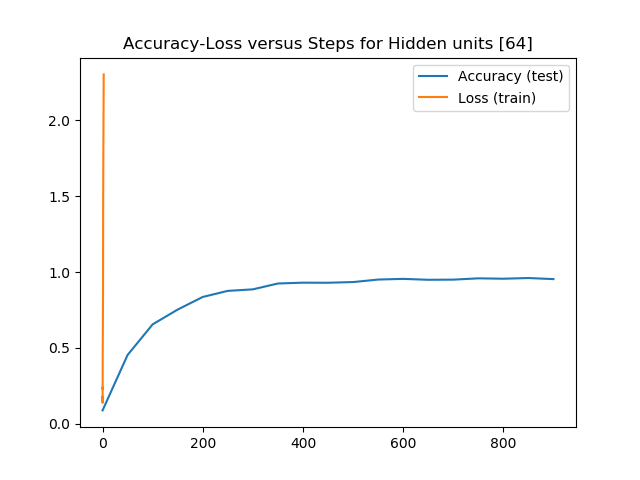
\includegraphics[angle=0,width=0.65\textwidth]{assign-3/logs/Q1-MNIST-LSTM-[64].png}
\caption{$H=64$, LSTM, Accuracy Loss Curves}
\end{subfigure}
\begin{subfigure}
\centering
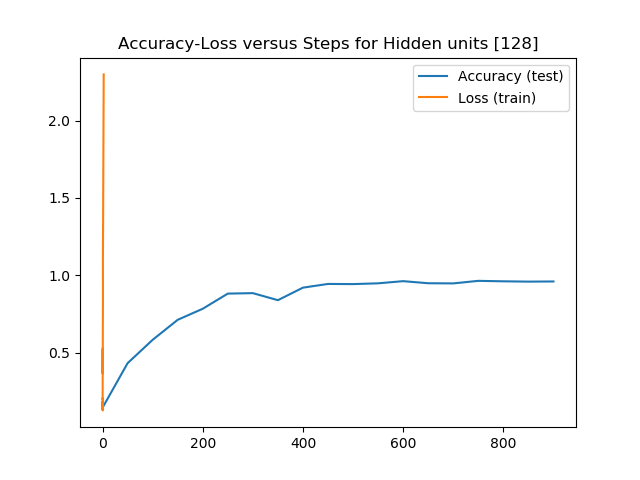
\includegraphics[angle=0,width=0.65\textwidth]{assign-3/logs/Q1-MNIST-LSTM-[128].png}
\caption{$H=128$, LSTM, Accuracy Loss Curves}
\end{subfigure}
\begin{subfigure}
\centering
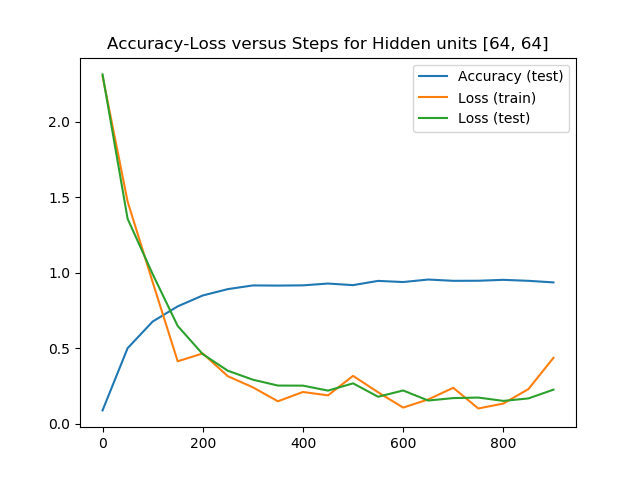
\includegraphics[angle=0,width=0.65\textwidth]{assign-3/logs/Q1-MNIST-LSTM-[64, 64].png}
\caption{$H=64, 128$, LSTM, Accuracy Loss Curves}
\end{subfigure}
\end{figure}
\begin{figure}[!htbp]
\begin{subfigure}
\centering
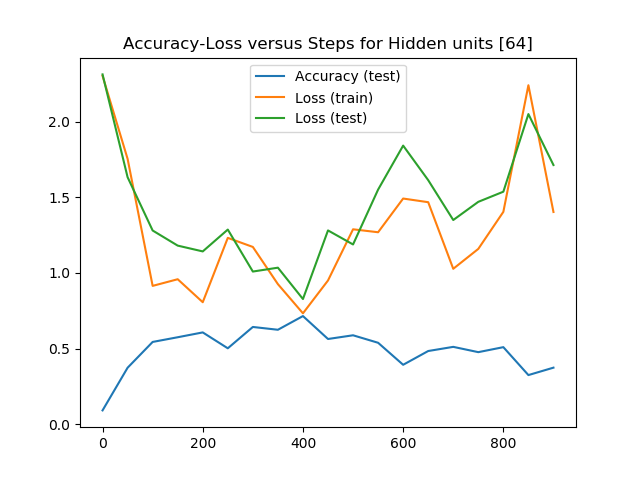
\includegraphics[angle=0,width=0.65\textwidth]{assign-3/logs/Q1-MNIST-RNN-[64].png}
\caption{$H=64$, RNN, Accuracy Loss Curves}
\end{subfigure}
\begin{subfigure}
\centering
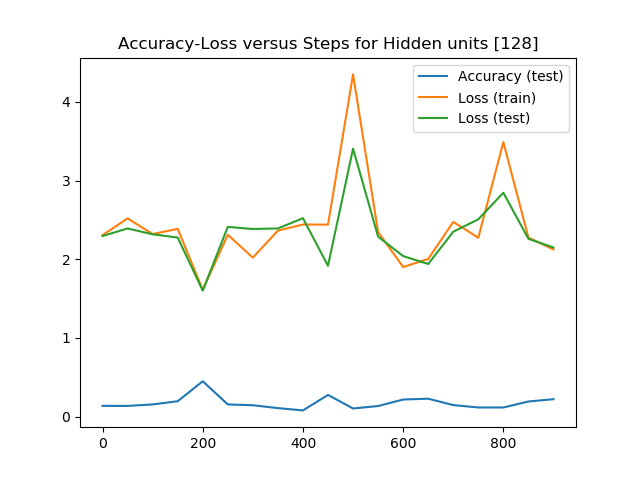
\includegraphics[angle=0,width=0.65\textwidth]{assign-3/logs/Q1-MNIST-RNN-[128].png}
\caption{$H=128$, RNN, Accuracy Loss Curves}
\end{subfigure}
\begin{subfigure}
\centering
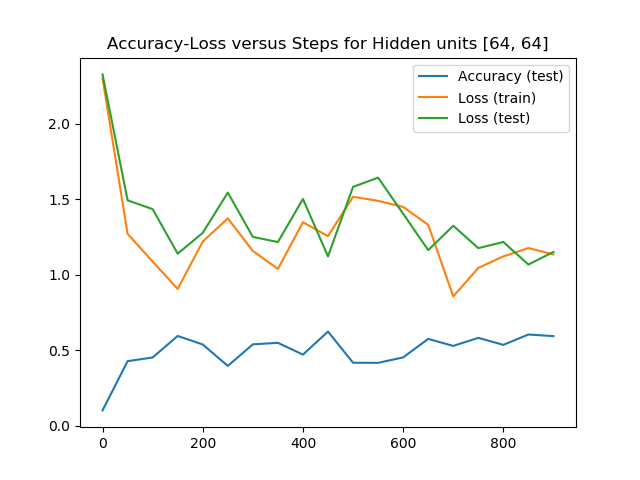
\includegraphics[angle=0,width=0.65\textwidth]{assign-3/logs/Q1-MNIST-RNN-[64, 64].png}
\caption{$H=64, 128$, RNN, Accuracy Loss Curves}
\end{subfigure}
\end{figure}
\begin{figure}[!htbp]
\begin{subfigure}
\centering
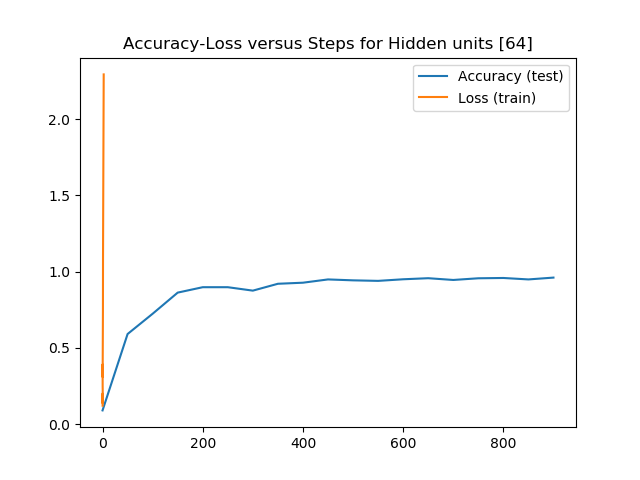
\includegraphics[angle=0,width=0.65\textwidth]{assign-3/logs/Q1-MNIST-GRU-[64].png}
\caption{$H=64$, GRU, Accuracy Loss Curves}
\end{subfigure}
\begin{subfigure}
\centering
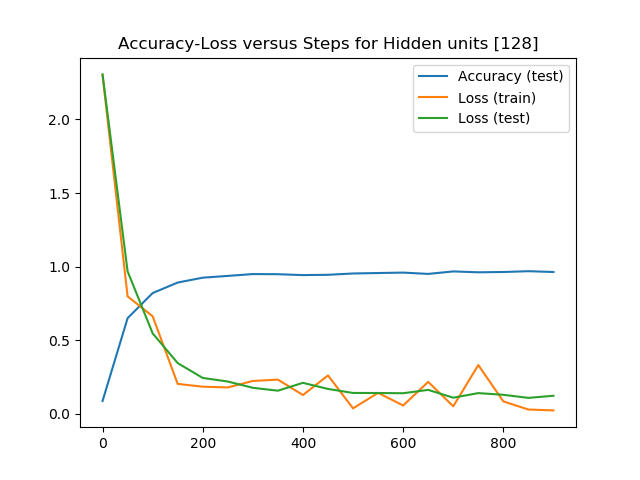
\includegraphics[angle=0,width=0.65\textwidth]{assign-3/logs/Q1-MNIST-GRU-[128].png}
\caption{$H=128$, GRU, Accuracy Loss Curves}
\end{subfigure}
\begin{subfigure}
\centering
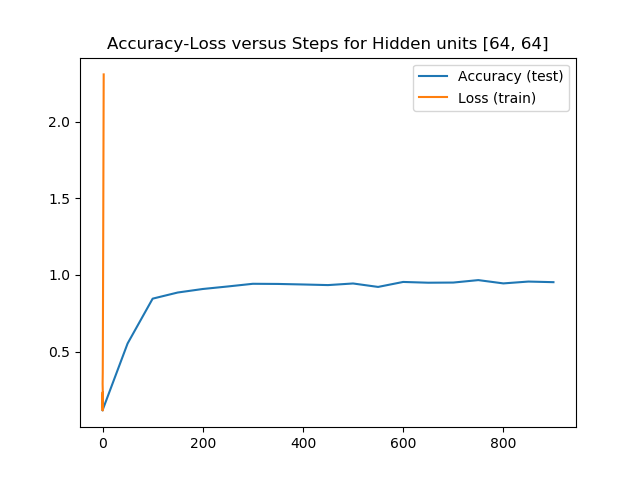
\includegraphics[angle=0,width=0.65\textwidth]{assign-3/logs/Q1-MNIST-GRU-[64, 64].png}
\caption{$H=64, 128$, GRU, Accuracy Loss Curves}
\end{subfigure}
\end{figure}

We also experiment with bi directional models.

\begin{figure}[!htbp]
\begin{subfigure}
\centering
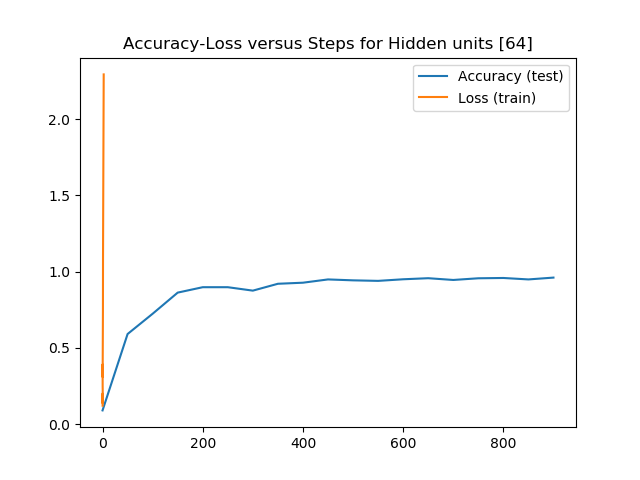
\includegraphics[angle=0,width=0.65\textwidth]{assign-3/logs/Q1-MNIST-GRU-[64].png}
\caption{$H=64$, GRU bidirectional, Accuracy Loss Curves}
\end{subfigure}
\begin{subfigure}
\centering
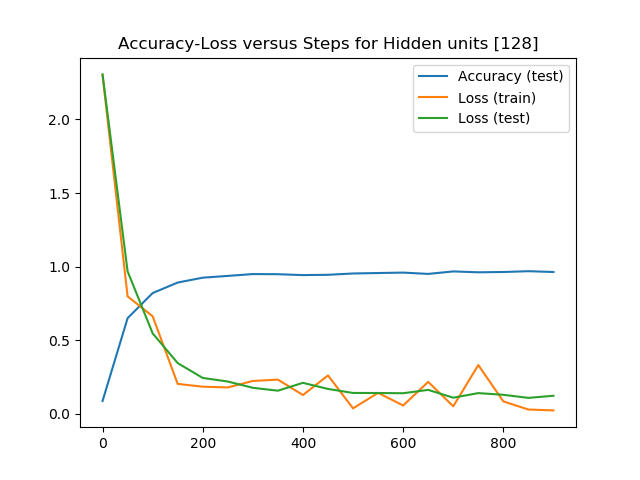
\includegraphics[angle=0,width=0.65\textwidth]{assign-3/logs/Q1-MNIST-GRU-[128].png}
\caption{$H=128$, GRU bidirectional, Accuracy Loss Curves}
\end{subfigure}
\begin{subfigure}
\centering
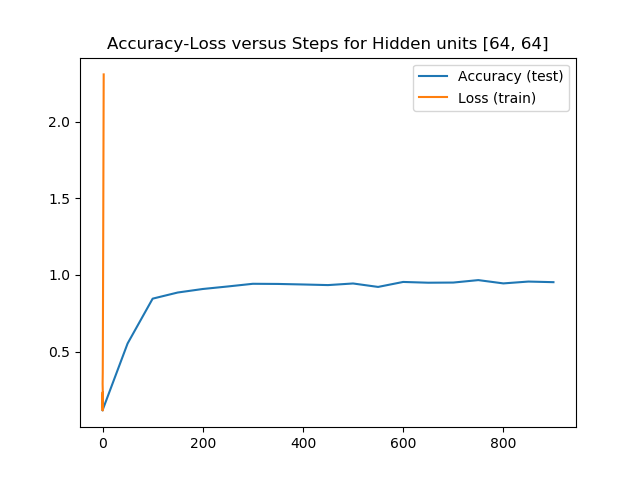
\includegraphics[angle=0,width=0.65\textwidth]{assign-3/logs/Q1-MNIST-GRU-[64, 64].png}
\caption{$H=64, 128$, GRU bidirectional, Accuracy Loss Curves}
\end{subfigure}
\end{figure}

\begin{figure}[!htbp]
\begin{subfigure}
\centering
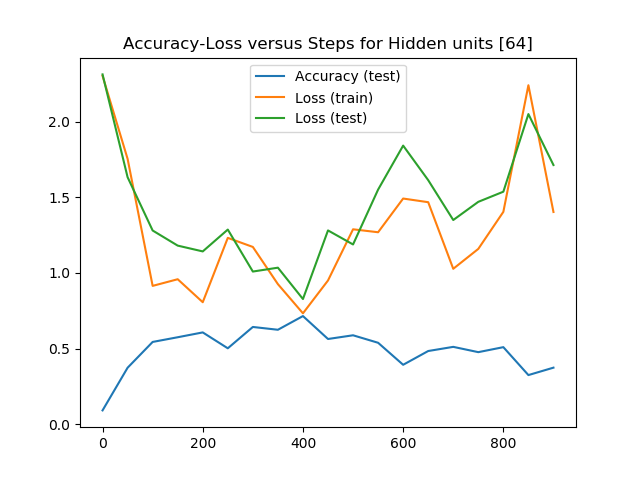
\includegraphics[angle=0,width=0.65\textwidth]{assign-3/logs/Q1-MNIST-RNN-[64].png}
\caption{$H=64$, RNN bidirectional, Accuracy Loss Curves}
\end{subfigure}
\begin{subfigure}
\centering
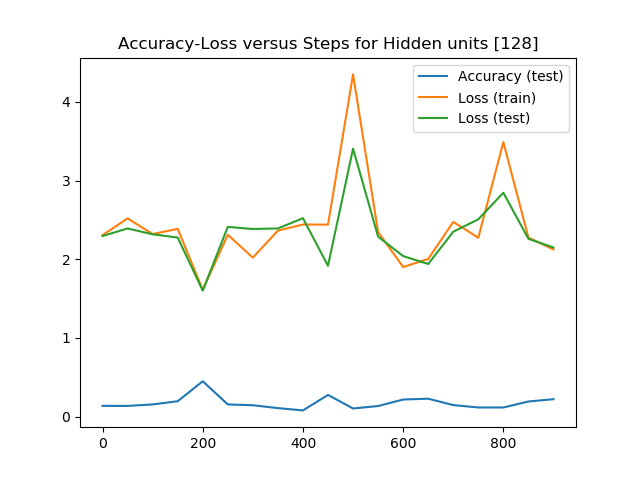
\includegraphics[angle=0,width=0.65\textwidth]{assign-3/logs/Q1-MNIST-RNN-[128].png}
\caption{$H=128$, RNN bidirectional, Accuracy Loss Curves}
\end{subfigure}
\begin{subfigure}
\centering
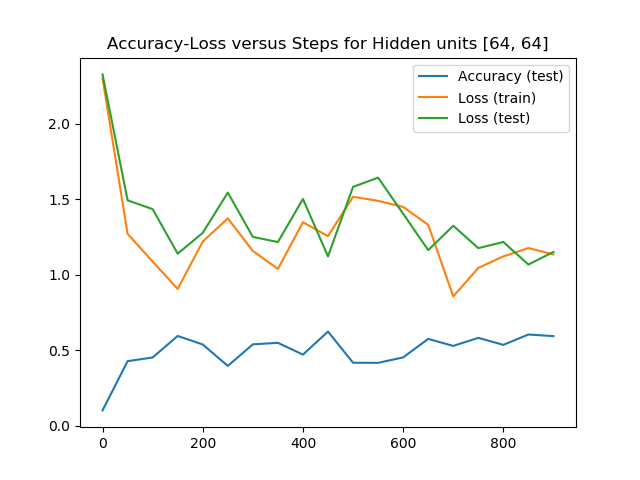
\includegraphics[angle=0,width=0.65\textwidth]{assign-3/logs/Q1-MNIST-RNN-[64, 64].pngg}
\caption{$H=64, 128$, RNN bidirectional, Accuracy Loss Curves}
\end{subfigure}
\end{figure}

\begin{figure}[!htbp]
\begin{subfigure}
\centering
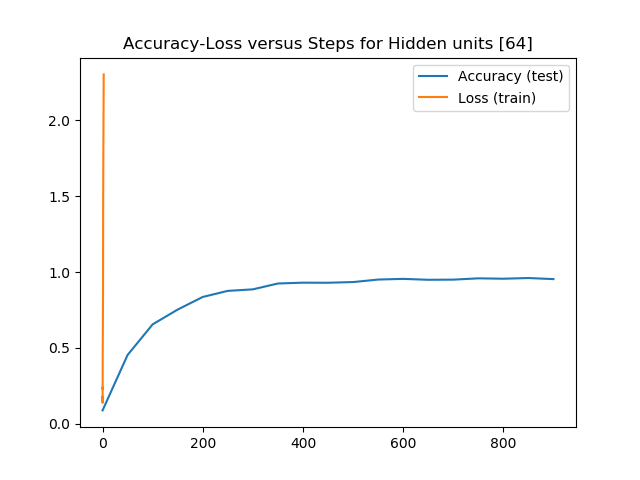
\includegraphics[angle=0,width=0.65\textwidth]{assign-3/logs/Q1-MNIST-LSTM-[64].png}
\caption{$H=64$, LSTM bidirectional, Accuracy Loss Curves}
\end{subfigure}
\begin{subfigure}
\centering
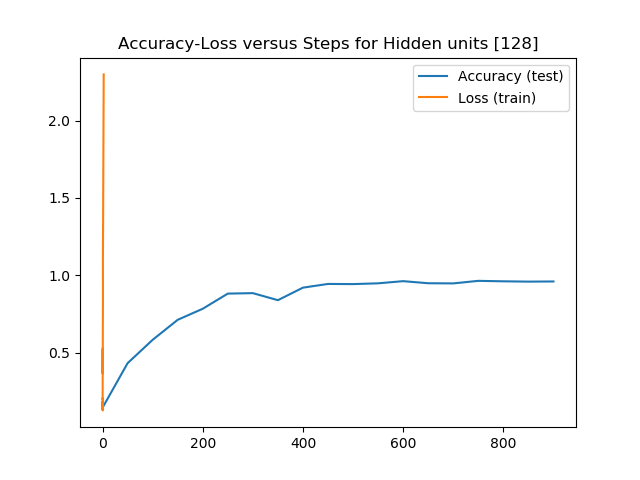
\includegraphics[angle=0,width=0.65\textwidth]{assign-3/logs/Q1-MNIST-LSTM-[128].png}
\caption{$H=128$, LSTM bidirectional, Accuracy Loss Curves}
\end{subfigure}
\begin{subfigure}
\centering
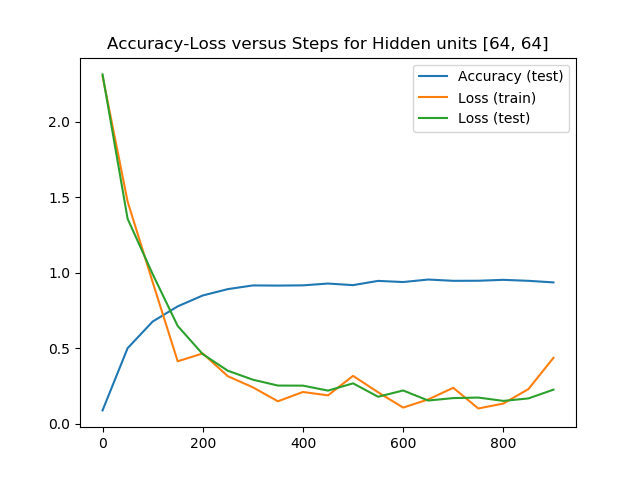
\includegraphics[angle=0,width=0.65\textwidth]{assign-3/logs/Q1-MNIST-LSTM-[64, 64].png}
\caption{$H=64, 128$, LSTM bidirectional, Accuracy Loss Curves}
\end{subfigure}
\end{figure}

\section{Question 2 }

We use a LSTM with the following hyper-parameters:

\begin{itemize}
\item  Adam optimiser, lr = 0.01, beta1 = 0.9, beta2 = 0.99
\item  Loss : Cross Entropy
\item  Single hidden layer, : 2,5,10 units wide.
\end{itemize}

The outputs of this question may be generated by:

\begin{lstlisting}
python3 q3.py --H 5
\end{lstlisting} 

We notice that increasing the hidden unit size increases the accuracy, due to better representation power.

We also perform randomised testing in the following format:\\
\begin{lstlisting}
Input Sequence tensor([[3, 5, 8, 6, 8]], dtype=torch.int32)
Truth tensor([5])
Prediction 5
\end{lstlisting}

\subsection{Loss and Accuracy Curves for H values}

\begin{figure}[!htbp]
\begin{subfigure}
\centering
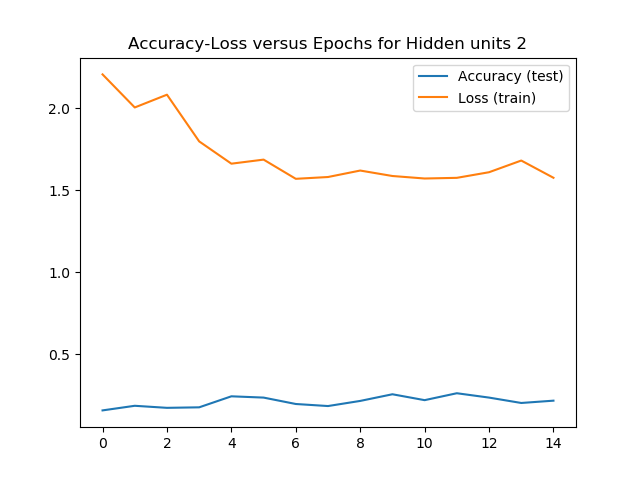
\includegraphics[angle=0,width=0.65\textwidth]{assign-3/logs/Q2-A-L-2.png}
\caption{$H=3$, Accuracy Loss Curves}
\end{subfigure}
\begin{subfigure}
\centering
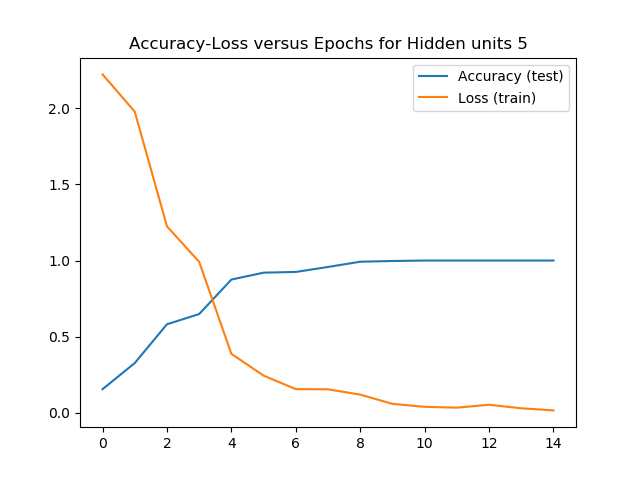
\includegraphics[angle=0,width=0.65\textwidth]{assign-3/logs/Q2-A-L-5.png}
\caption{$H=5$, Accuracy Loss Curves}
\end{subfigure}
\begin{subfigure}
\centering
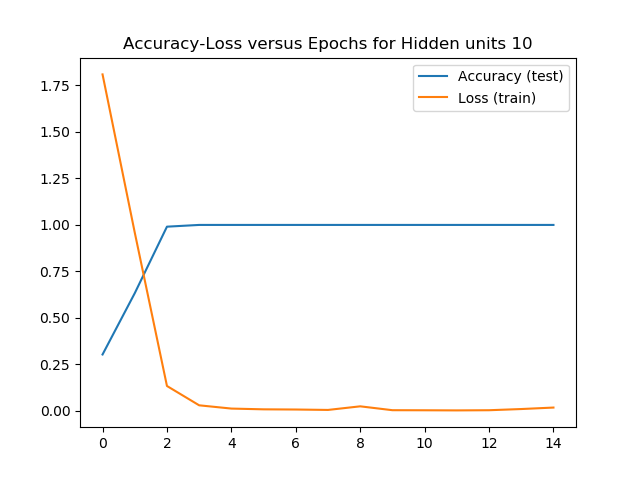
\includegraphics[angle=0,width=0.65\textwidth]{assign-3/logs/Q2-A-L-10.png}
\caption{$H=10$,Accuracy Loss Curves}
\end{subfigure}
\end{figure}

\section{Question 3}

We use a LSTM for this question with hidden (state) size as 5. We notice that increasing this to 10 improves accuracy (nearly 100\%) and decreasing to 2 lowers accuracy. These plots however, aren't included here, and we experiment with state size 5.

The outputs of this question may be generated by:

\begin{lstlisting}
python3 q3.py --loss_type MSE
\end{lstlisting} 

Hyper-parameters:
\begin{itemize}
\item  Adam optimiser, lr = 0.01, beta1 = 0.9, beta2 = 0.99
\item  Loss : MSE and Cross Entropy
\item  Single hidden layer, 5 units wide.
\end{itemize}

\subsection{MSE vs Cross Entropy}

We also note that MSE performs much better than Cross Entropy. This is because the output sequence is a binary number and their probabilities are correlated. Hence, we cannot use a "clean" version of cross entropy with $L$ distinct distributions. We use a hackish method to use cross entropy, and for the reasons noted above, it performs poorly. We plot validation in blue, train in orange.

\begin{figure}[!htbp]
\begin{subfigure}
\centering
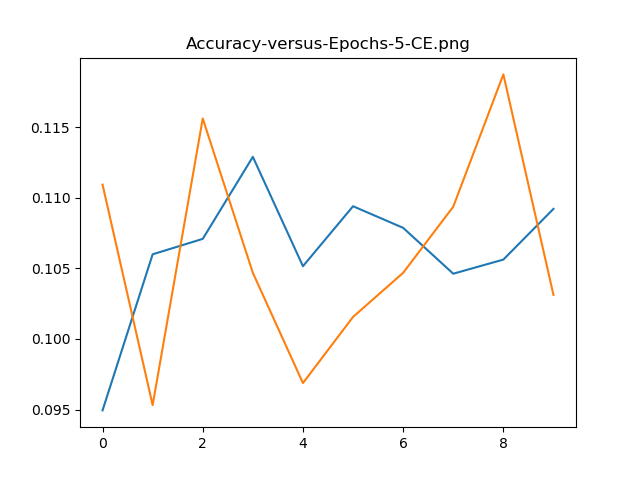
\includegraphics[angle=0,width=0.65\textwidth]{assign-3/logs/Accuracy-5-CE-hidden-5.png}
\caption{$L=5$, Cross Entropy Loss}
\end{subfigure}
\begin{subfigure}
\centering
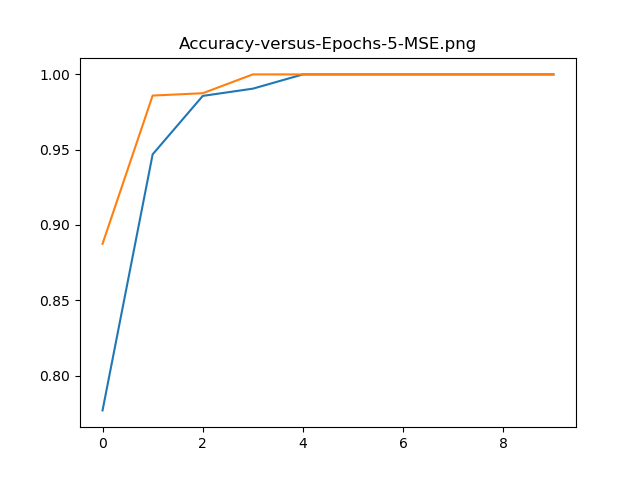
\includegraphics[angle=0,width=0.65\textwidth]{assign-3/logs/Accuracy-5-MSE-hidden-5.png}
\caption{$L=5$, MSE Loss}
\end{subfigure}
\end{figure}

\begin{figure}[!htbp]
\begin{subfigure}
\centering
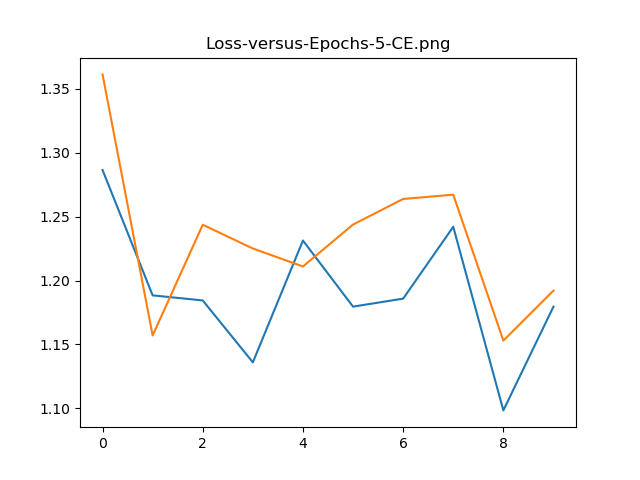
\includegraphics[angle=0,width=0.65\textwidth]{assign-3/logs/Loss-5-CE-hidden-5.png}
\caption{$L=5$, Cross Entropy Loss}
\end{subfigure}
\begin{subfigure}
\centering
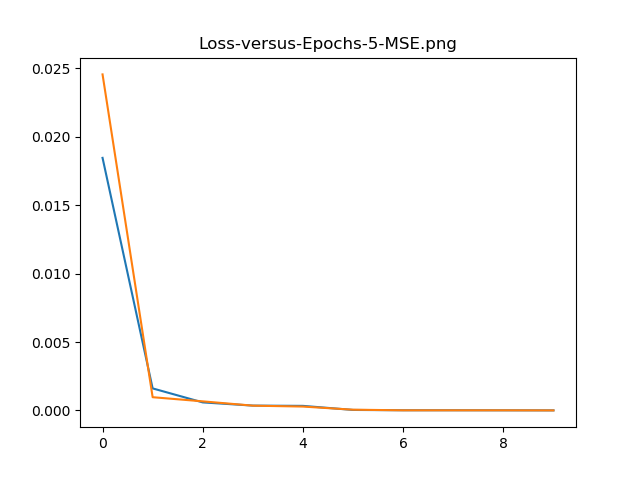
\includegraphics[angle=0,width=0.65\textwidth]{assign-3/logs/Loss-5-MSE-hidden-5.png}
\caption{$L=5$, MSE Loss}
\end{subfigure}
\end{figure}

\subsection{MSE: Loss and Accuracy Curves}

We include loss and accuracy curves for all sequence lengths (3,5,10) used.

\begin{figure}[!htbp]
\begin{subfigure}
\centering
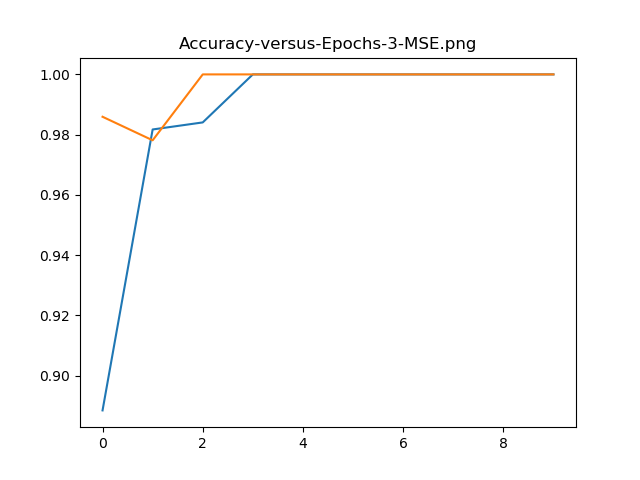
\includegraphics[angle=0,width=0.65\textwidth]{assign-3/logs/Accuracy-3-MSE-hidden-5.png}
\caption{$L=3$, Accuracy, MSE}
\end{subfigure}
\begin{subfigure}
\centering
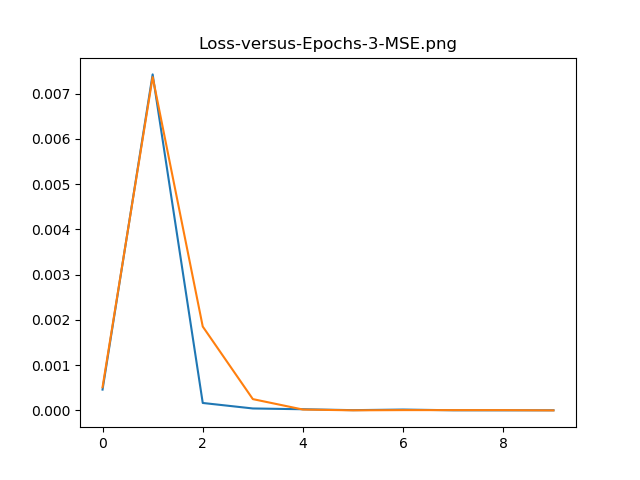
\includegraphics[angle=0,width=0.65\textwidth]{assign-3/logs/Loss-3-MSE-hidden-5.png}
\caption{$L=3$, Loss , MSE}
\end{subfigure}
\end{figure}

\begin{figure}[!htbp]
\begin{subfigure}
\centering
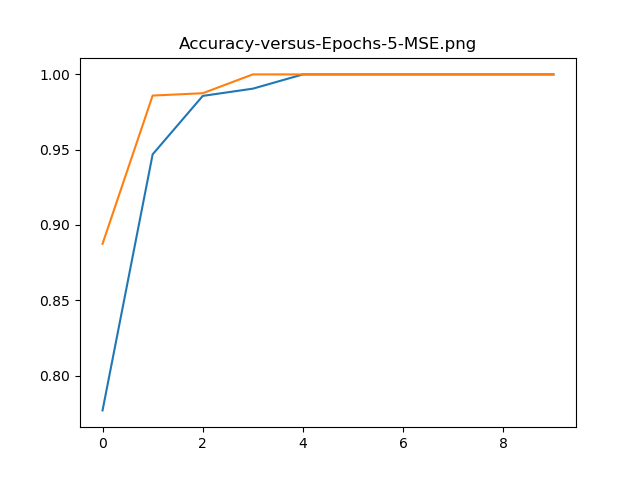
\includegraphics[angle=0,width=0.65\textwidth]{assign-3/logs/Accuracy-5-MSE-hidden-5.png}
\caption{$L=5$, Accuracy, MSE}
\end{subfigure}
\begin{subfigure}
\centering
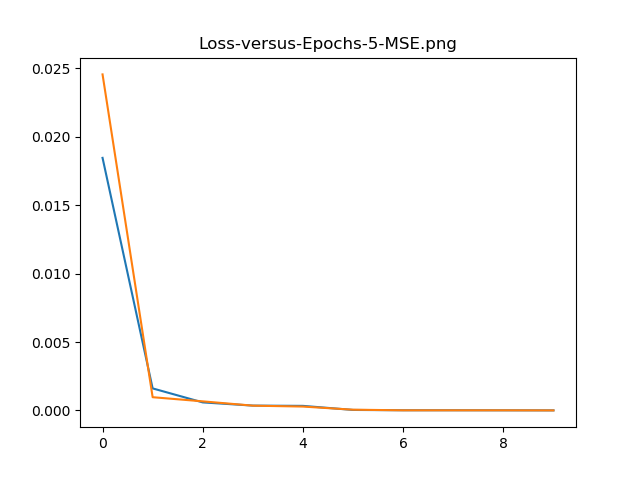
\includegraphics[angle=0,width=0.65\textwidth]{assign-3/logs/Loss-5-MSE-hidden-5.png}
\caption{$L=5$, Loss, MSE}
\end{subfigure}
\end{figure}

\begin{figure}[!htbp]
\begin{subfigure}
\centering
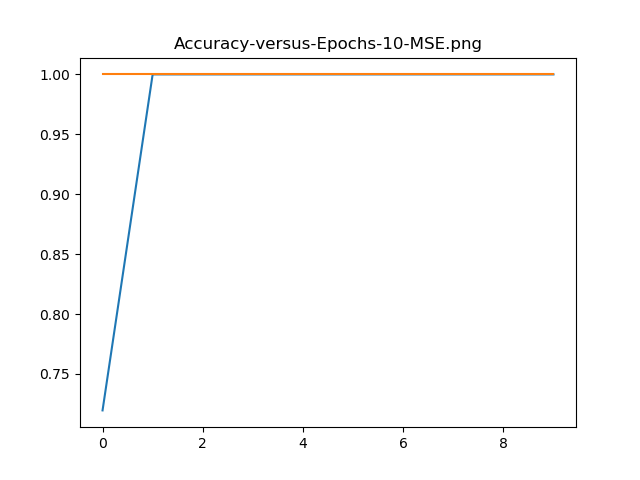
\includegraphics[angle=0,width=0.65\textwidth]{assign-3/logs/Accuracy-10-MSE-hidden-5.png}
\caption{$L=10$, Accuracy, MSE}
\end{subfigure}
\begin{subfigure}
\centering
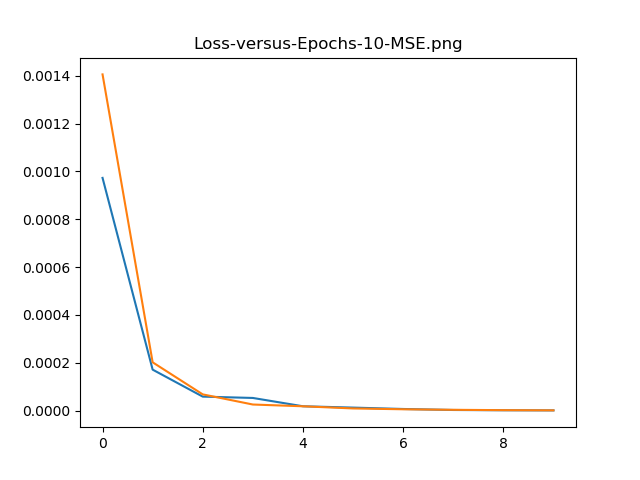
\includegraphics[angle=0,width=0.65\textwidth]{assign-3/logs/Loss-10-MSE-hidden-5.png}
\caption{$L=10$, Loss, MSE}
\end{subfigure}
\end{figure}

\subsection{MSE: Average Bit accuracy}

We perform this for $L=3, 5, 10$ as the training data.

\begin{figure}[!htbp]
\begin{subfigure}
\centering
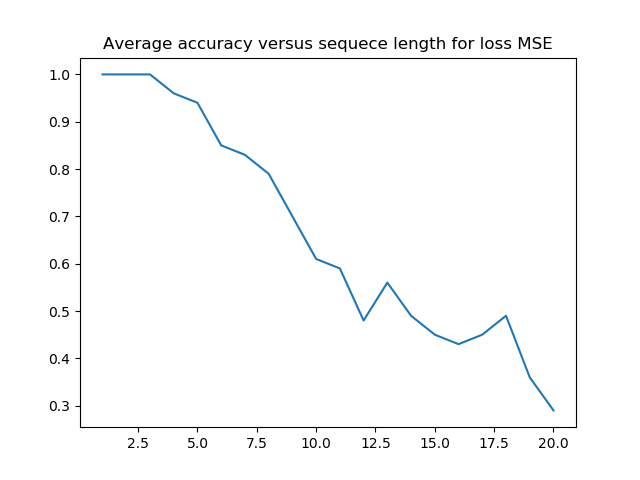
\includegraphics[angle=0,width=0.65\textwidth]{assign-3/logs/AV-Loss-3-MSE-hidden-5.png}
\caption{$L=3$, Average Bit rate Loss}
\end{subfigure}
\begin{subfigure}
\centering
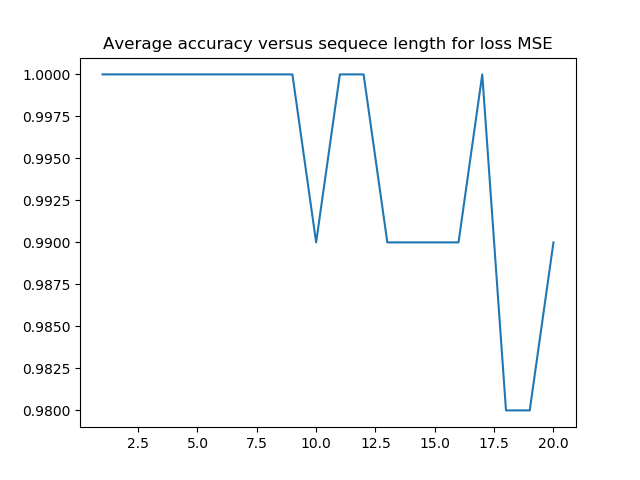
\includegraphics[angle=0,width=0.65\textwidth]{assign-3/logs/AV-Loss-5-MSE-hidden-5.png}
\caption{$L=5$, Average Bit rate Loss}
\end{subfigure}
\begin{subfigure}
\centering
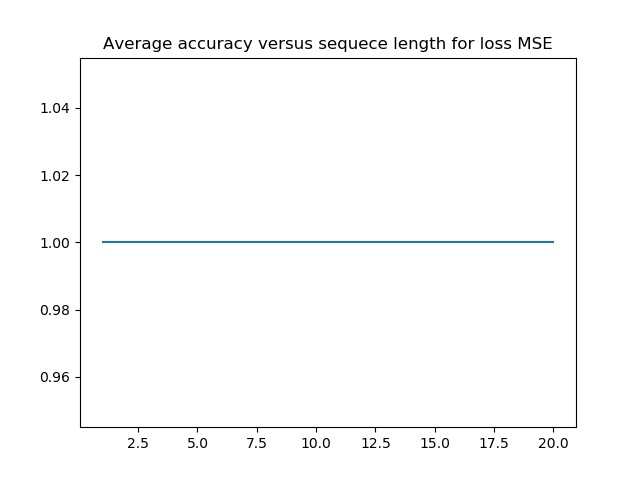
\includegraphics[angle=0,width=0.65\textwidth]{assign-3/logs/AV-Loss-10-MSE-hidden-5.png}
\caption{$L=10$, Average Bit rate Loss}
\end{subfigure}
\end{figure}






 